\begin{abstract}
\noindent
Malware in the browser can change the recipient or amount of a bank transfer
while the screen still shows what the user typed; an ordinary one-time password
does not stop this. We build a demo bank with four interchangeable
authentication modes --- \texttt{baseline} (TOTP), \texttt{hmac} (a code over the
exact transaction), \texttt{sig} (an ECDSA signature over it) and
\texttt{sig\_blind} (the same signature with no phone display) --- and compare
them under one threat model with an automated harness of 14 attack-scenario
variants. Transaction binding blocks the tampering that \texttt{baseline} lets
through; signatures additionally survive a database leak and give
third-party--verifiable evidence; and blind signing shows that strong
cryptography fails without a trusted display.
\end{abstract}

\section{Introduction}\label{sec:main-intro}
A bank customer authenticates to the bank, but the device carrying their intent
--- the browser on a personal computer --- is not trustworthy. A
man-in-the-browser (MitB) Trojan can rewrite every request and response: the
customer asks to pay account~A, the Trojan sends account~B, and the page still
shows~A. A real-time phishing proxy reaches the same position from the network.
A one-time password (OTP) does not help, because it proves that the right person
is present but not \emph{which} transaction is approved; the attacker simply
uses it to authorise the tampered transfer.

The defence studied here is \emph{transaction binding}: the code or signature the
customer returns is computed over the exact transaction, and the transaction is
shown on a second, trusted device (the phone) so that the customer signs what
they see (WYSIWYS). The idea is long established~\cite{hiltgen2006,ztic2008}:
chipTAN and photoTAN derive a code from the transaction, OCRA defines a signature
mode~\cite{rfc6287}, EU Regulation 2018/389 mandates ``dynamic linking'' of the
code to amount and payee~\cite{eu2018389}, and W3C Secure Payment Confirmation
signs the transaction details~\cite{w3cspc}. User studies, however, show that
people do not always check the trusted display~\cite{alzomai2008,haupert2019}.

We therefore do not propose a new mechanism. We implement four modes on one code
base --- a plain TOTP (\texttt{baseline})~\cite{rfc4226,rfc6238}, a
transaction-bound HMAC code (\texttt{hmac}), a transaction-bound ECDSA signature
(\texttt{sig}), and the same signature with no details shown on the phone
(\texttt{sig\_blind}) --- and compare them under one threat model. We ask three
questions. \textbf{RQ1:} does binding the code to the transaction stop MitB and
real-time phishing better than an ordinary OTP? \textbf{RQ2:} how do symmetric
and asymmetric binding differ in security and cost? \textbf{RQ3:} what does the
trusted display contribute, independently of the cryptography?

\section{Threat Model and Security Goals}\label{sec:main-threat}
We assume TLS is secure, the bank server is honest but its database may leak,
the phone is trusted and separate from the PC, and enrolment happens in a clean
environment. In scope are five attacker capabilities: a man-in-the-browser (A1);
a real-time phishing proxy (A2), which in this model can do exactly what A1 does
and is therefore covered by the same scenarios rather than a separate
experiment; replay (A3); online guessing (A4); and database theft (A5). Malware
on the phone (A6) and social engineering (A7) are out of scope; the literature
shows the phone--PC separation is fragile~\cite{dmitrienko2014,konoth2016,haupert2018}.

The modes are measured against seven goals: \textbf{G1}~authorization integrity
(the server executes $T$ only if the device produced a code for exactly $T$);
\textbf{G2}~freshness; \textbf{G3}~single use, even under concurrency;
\textbf{G4}~a guessing limit per transaction; \textbf{G5}~resilience to a
database leak; \textbf{G6}~verifiable evidence that a third party can check; and
\textbf{G7}~WYSIWYS for an attentive user.

\section{Design and Implementation}\label{sec:main-design}
The system has three parts: a FastAPI bank server with an SQLite database, a
browser-based phone authenticator, and a shared cryptographic core
(\texttt{tba\_core}). The PC browser is untrusted; the only channel from it to
the phone is a QR code, and the phone talks to the server over its own HTTPS
connection (\cref{fig:arch}).

\begin{figure}[htbp]
\centering
\resizebox{0.85\linewidth}{!}{%
\begin{tikzpicture}[
  font=\small,
  box/.style={draw,rounded corners,align=center,minimum height=9mm,inner sep=4pt},
  trusted/.style={box,fill=green!8},
  untrusted/.style={box,fill=red!8},
  neutral/.style={box,fill=blue!6},
  elab/.style={font=\scriptsize,fill=white,inner sep=1.5pt},
  >=Latex,node distance=10mm]
  % untrusted PC
  \node[untrusted] (br) {Browser\\(bank pages)};
  \node[untrusted,below=8mm of br] (mitb) {MitB\\\texttt{mitb\_addon.py}};
  % server
  \node[trusted,right=46mm of br] (web) {\texttt{server/app.py}\\routes + templates};
  \node[trusted,below=8mm of web] (ver) {\texttt{verify.py},\\\texttt{transfers.py},\\\texttt{auth.py}};
  \node[trusted,below=8mm of ver] (db) {SQLite};
  % phone
  \node[trusted,above=14mm of web] (app) {Phone authenticator\\Web Crypto + IndexedDB};
  % core / eval
  \node[neutral,right=28mm of ver] (core) {\texttt{tba\_core}\\encoding, totp,\\hmac\_otp, signature};
  \node[neutral,below=8mm of core] (eval) {\texttt{evaluation}\\harness, VirtualPhone,\\scenarios, bench};
  % edges
  \draw[->] (br) -- node[elab]{HTTPS} (mitb);
  \draw[->] (mitb.east) -- node[elab,below]{HTTPS} (web.west|-mitb.east);
  \draw[->] (app) -- node[elab]{HTTPS} (web);
  \draw[->,dashed] (app.west) to[bend right=20] node[elab,left]{QR on screen} (br.north);
  \draw[->] (web) -- (ver);
  \draw[->] (ver) -- (db);
  \draw[->] (ver) -- (core);
  \draw[->] (eval) -- (core);
  \draw[->] (eval.north) to[bend right=12] node[elab,right]{TestClient} (web.south);
\end{tikzpicture}}
\caption{Architecture and trust boundaries. Green: trusted; red: untrusted;
blue: test/verification code. The QR code is the only channel from the
untrusted browser to the trusted phone, and the phone talks to the server on its
own HTTPS channel.}
\label{fig:arch}
\end{figure}

\paragraph{Canonical transaction.}
A transaction is a fixed JSON object (\texttt{tx\_id}, sender, recipient
account and name, amount, currency, a 16-byte nonce, and an expiry 120~s after
creation). Both sides serialise it to identical bytes: sorted keys, no
whitespace, ASCII only, with strict parsing that rejects duplicate keys, floats
and any non-canonical input. A suite of 20 JavaScript tests checks the phone's
implementation against test vectors shared with the Python server. The server always
verifies against the canonical transaction stored in its \emph{own} database,
never one supplied by the client.

\paragraph{The four modes.}
\texttt{baseline} computes a 6-digit TOTP (HMAC-SHA1, 30~s step), accepted
within $\pm1$ step and never twice. \texttt{hmac} computes an 8-digit truncation
of $\mathrm{HMAC\text{-}SHA256}(K, \text{tag}\,\|\,\texttt{0x00}\,\|\,\mathrm{canon}(tx))$,
compared in constant time. \texttt{sig} and \texttt{sig\_blind} compute an
ECDSA~P-256 signature over the same tagged bytes, sent as raw 64-byte $r\|s$ and
verified with the device's public key. The domain-separation tags stop a code
for one purpose being reused for another. The signing key is generated on the
phone with Web Crypto as a non-extractable key and is never sent to the server.

\paragraph{Enrolment and confirmation.}
Each user enrols one device by scanning a QR code; once a device exists the
server refuses a second enrolment (HTTP~409), otherwise an attacker with only a
web session could enrol their own key. Each confirmation runs inside one
\texttt{BEGIN IMMEDIATE} database transaction: the server checks ownership,
state and expiry, verifies the code or signature, counts failures (three
failures lock the transaction), and only then moves the balances and stores the
evidence.

\section{Security Evaluation}\label{sec:main-eval}
The evaluation is automated: a fresh in-process server, a virtual phone built
on \texttt{tba\_core}, and a simulated MitB that rewrites requests and QR codes
exactly as our live \texttt{mitmproxy} addon does. An \emph{attentive} user
approves only when the phone display matches their intent --- and, having
nothing to compare, also approves when the phone shows no details
(\texttt{sig\_blind}); a \emph{careless} user always approves. The 14 scenario
variants (S1--S13, with S2 split by user model) run in all four modes, and each
outcome is compared with a pre-declared expected value; measured and expected
outcomes agree in all 56 cells (\cref{tab:scenarios}). Most scenarios run
against the in-process server; S5 and S12 exercise the cryptographic library
directly, S8 tests the confirmation logic under concurrent database
connections, and S13 sends malformed signatures over HTTP.

\begin{table}[htbp]
\centering
\caption{Scenario outcomes across the four modes (\cmark{} secure, \xmark{}
insecure, -- not applicable). Source: \texttt{results/scenarios.csv}.}
\label{tab:scenarios}
\small
\begin{tabularx}{\linewidth}{@{}lXcccc@{}}
\toprule
ID & Scenario & baseline & hmac & sig & sig\_blind \\
\midrule
S1 & Honest transfer & \cmark & \cmark & \cmark & \cmark \\
S2a & MitB swaps recipient, attentive user & \xmark & \cmark & \cmark & \xmark \\
S2b & MitB swaps recipient, careless user & \xmark & \xmark & \xmark & \xmark \\
S3 & MitB changes amount & \xmark & \cmark & \cmark & \xmark \\
S4 & MitB forges QR with intended details & \xmark & \cmark & \cmark & \cmark \\
S5 & Tamper each field after code issued & \xmark & \cmark & \cmark & \cmark \\
S6 & Replay code on old and new transaction & \cmark & \cmark & \cmark & \cmark \\
S7 & Confirm after expiry & \cmark & \cmark & \cmark & \cmark \\
S8 & 50 concurrent submissions of one code & \cmark & \cmark & \cmark & \cmark \\
S9 & 3 wrong guesses, then correct code & \cmark & \cmark & \cmark & \cmark \\
S10 & Server DB leak, forge transfer & \xmark & \xmark & \cmark & \cmark \\
S11 & Third party can verify evidence & \xmark & \xmark & \cmark & \cmark$^{*}$ \\
S12 & Non-canonical QR payloads & -- & \cmark & \cmark & \cmark \\
S13 & Malformed signatures & -- & -- & \cmark & \cmark \\
\bottomrule
\end{tabularx}
\par\smallskip{\footnotesize $^{*}$ The signature proves that the device signed, not that the user saw the transaction.\par}
\end{table}

\paragraph{RQ1: binding.}
\texttt{baseline} fails every tampering scenario (S2a, S3, S4, S5): the stolen
code authorises whatever transaction the server holds. \texttt{hmac} and
\texttt{sig} block all four, because a code for one transaction does not verify
for another and the phone shows the true recipient. In the live MitB demo the
laptop shows the intended recipient in every mode while the phone shows the
attacker's account (\cref{fig:mitb}). By the A1/A2 equivalence the same holds
for real-time phishing.

\begin{figure}[htbp]
\centering
\begin{minipage}{0.3\linewidth}\centering
  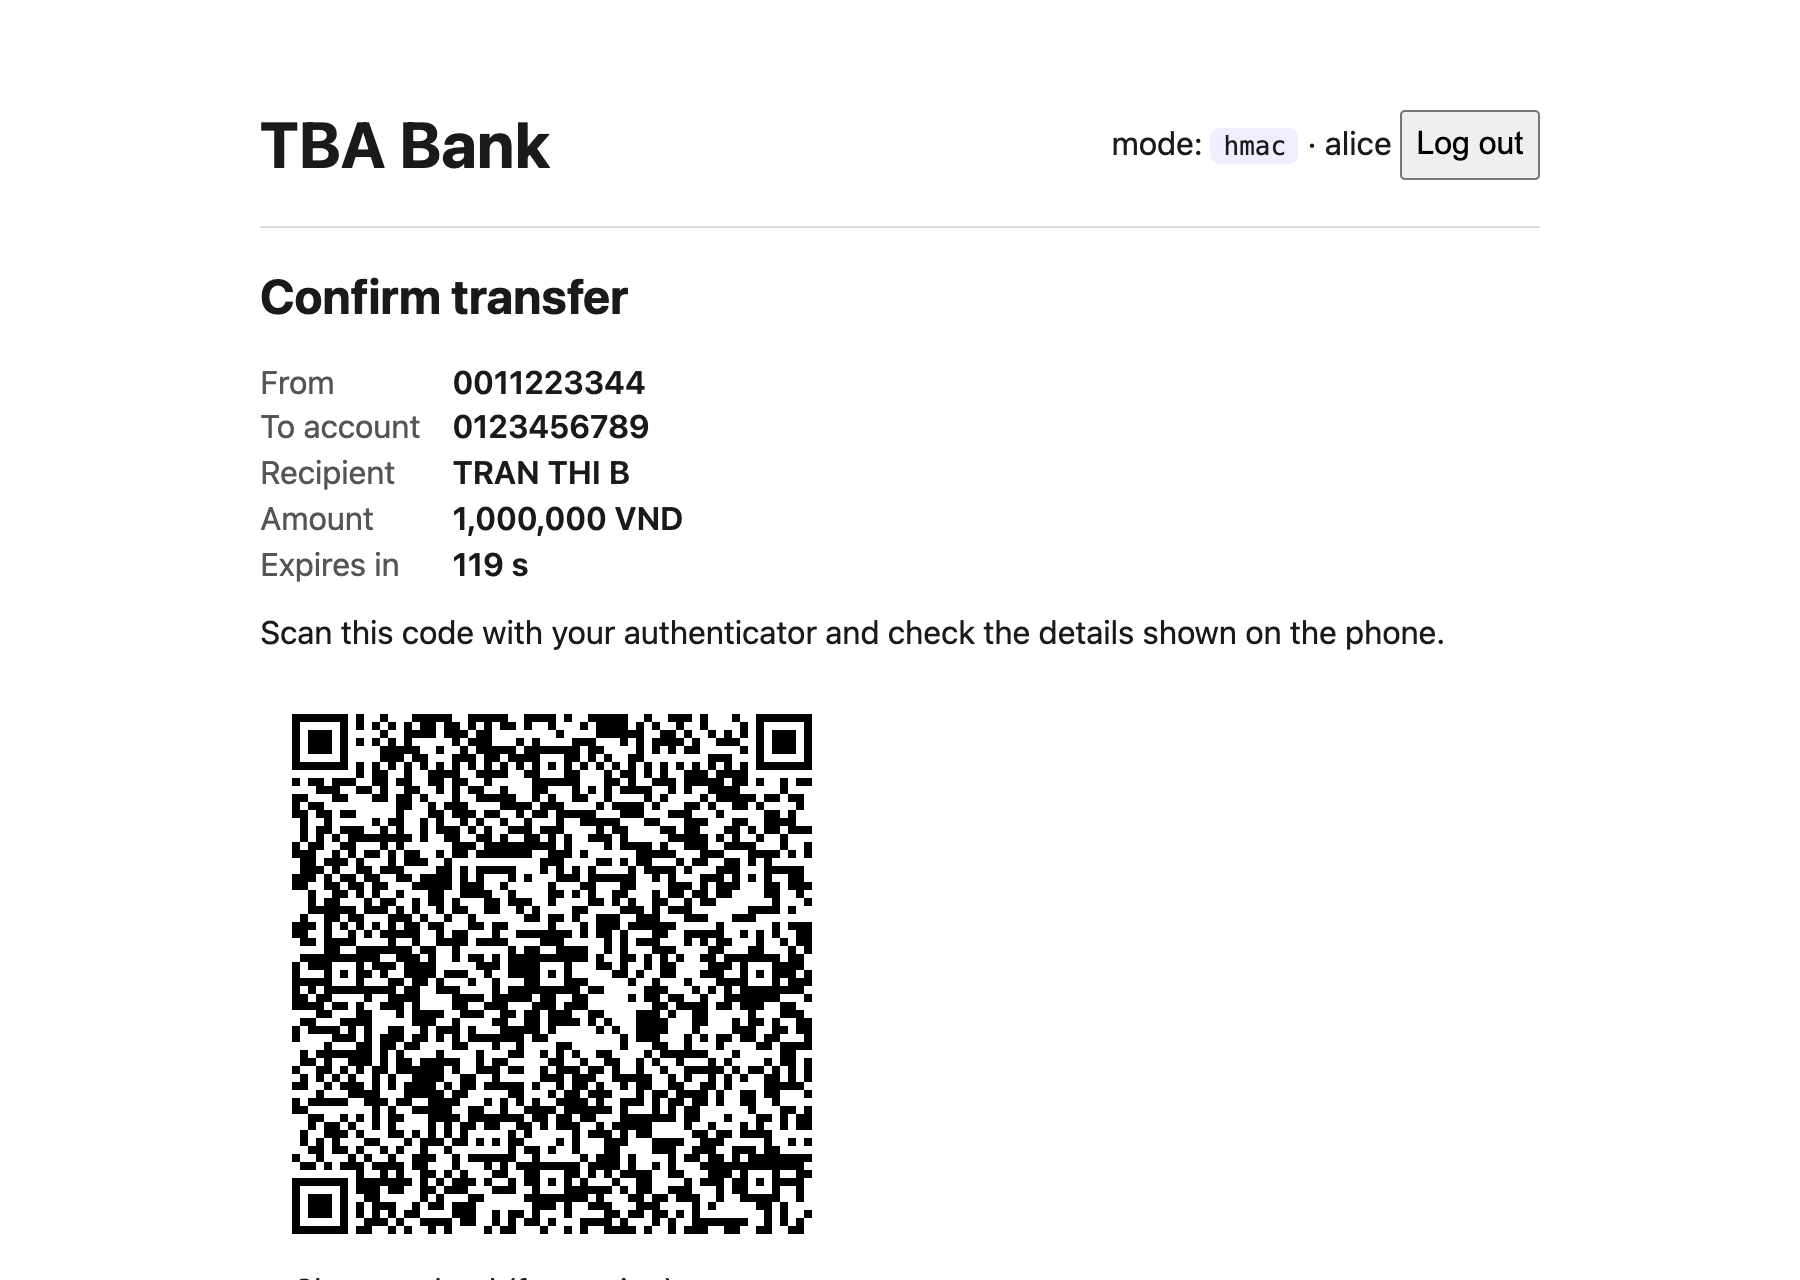
\includegraphics[width=\linewidth]{figures/hmac_laptop.png}\\[1mm]
  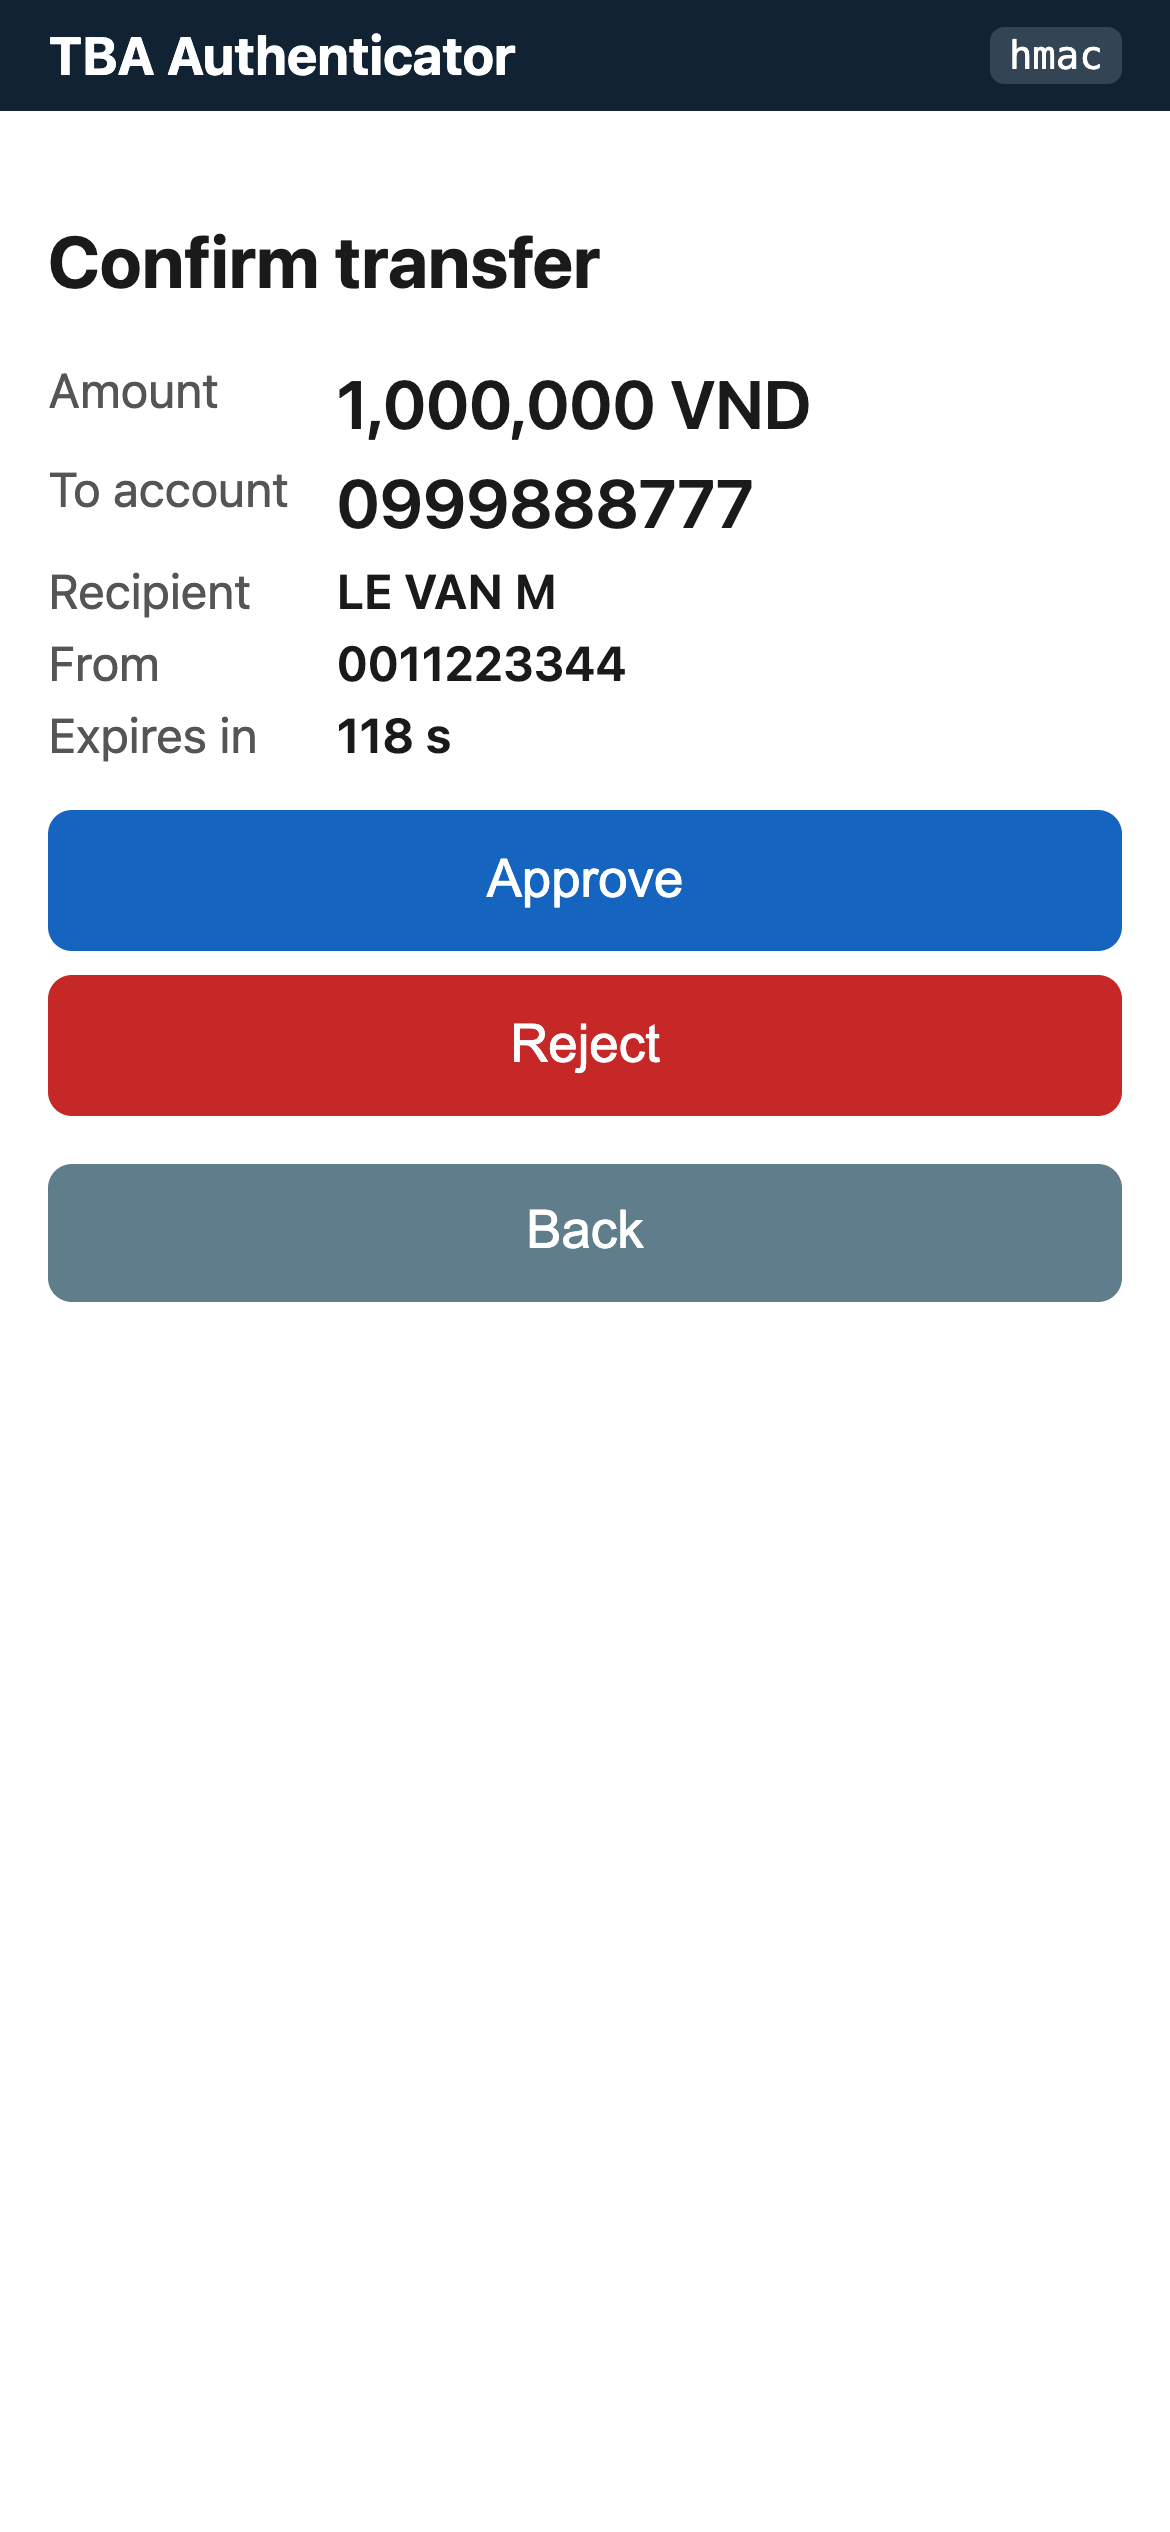
\includegraphics[height=3.4cm]{figures/hmac_phone.png}\\ \footnotesize\texttt{hmac}
\end{minipage}\hfill
\begin{minipage}{0.3\linewidth}\centering
  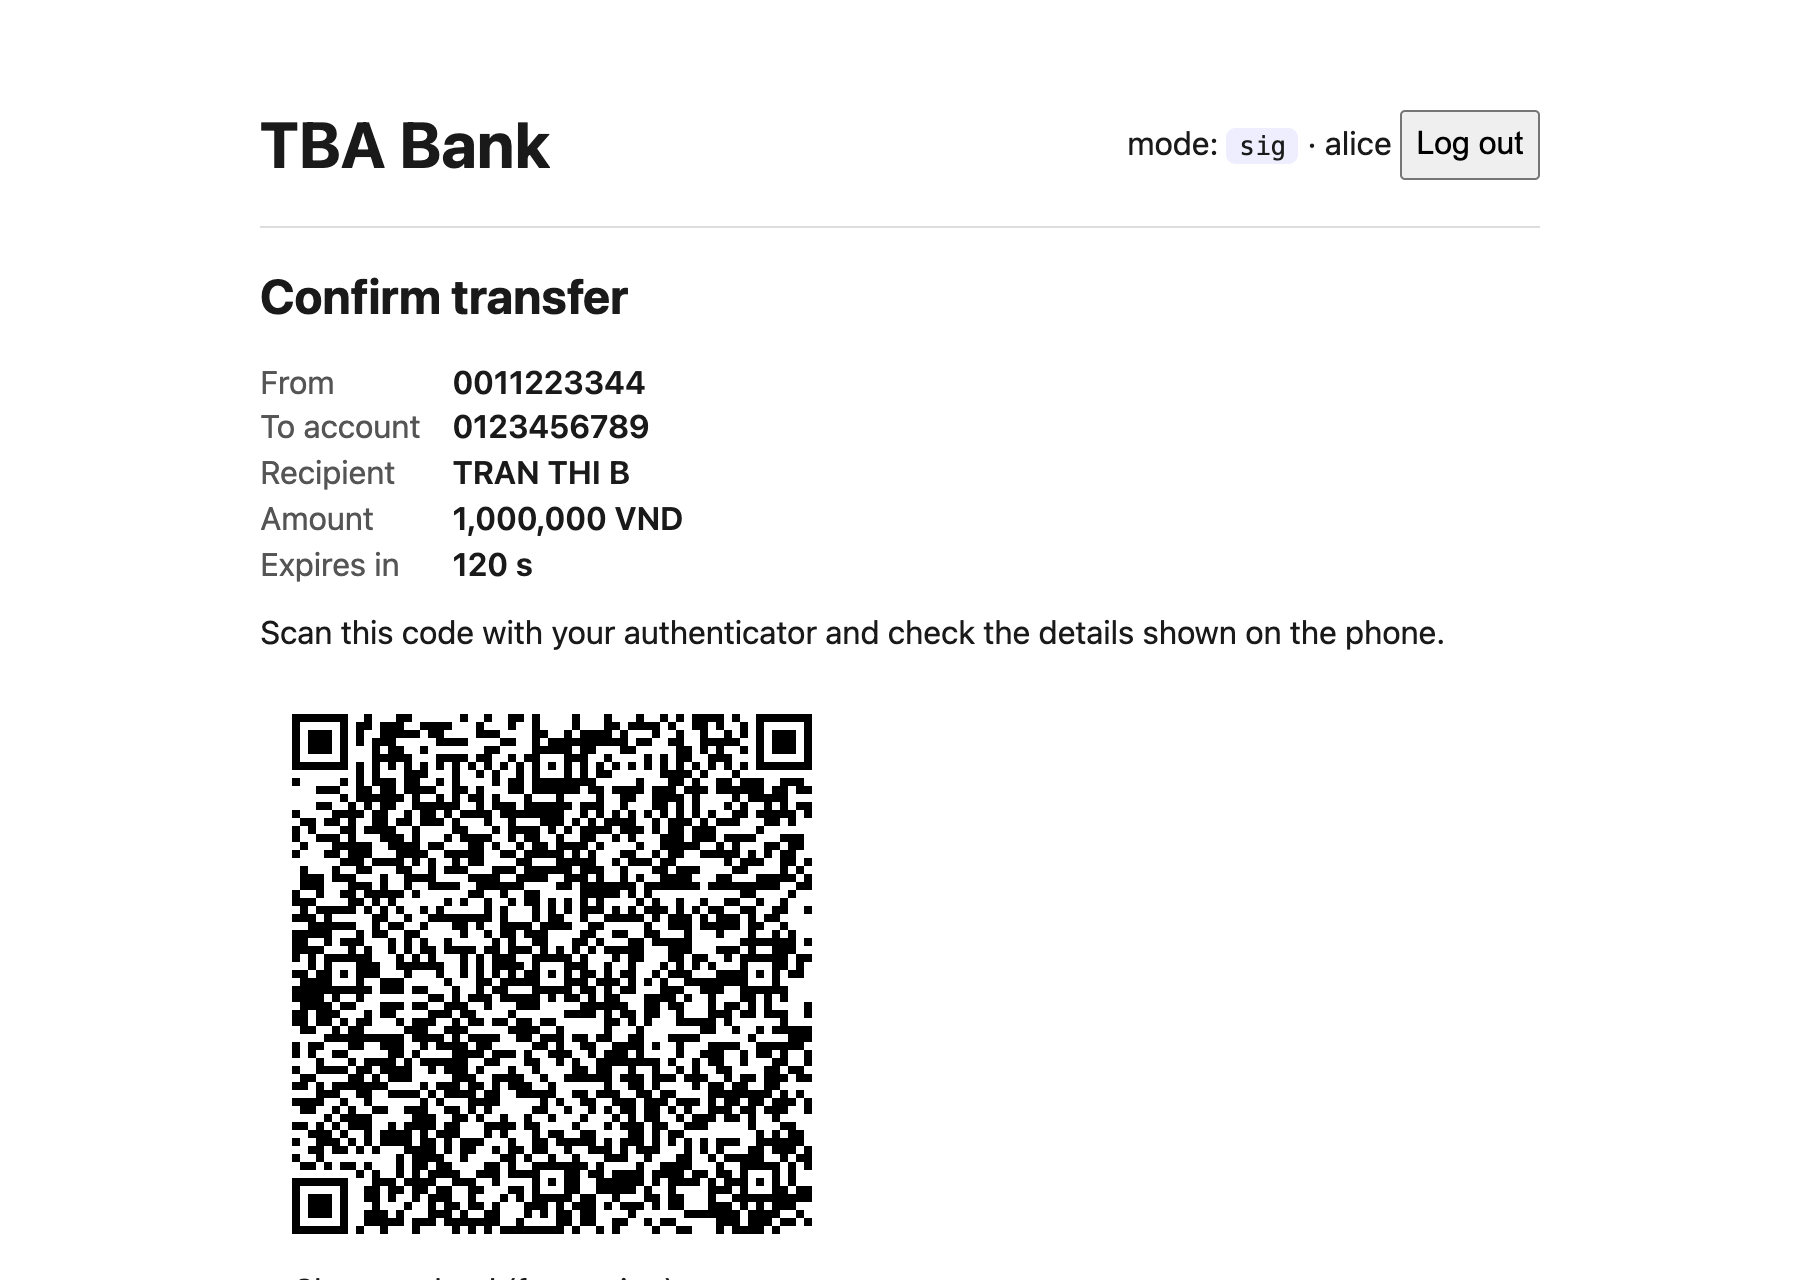
\includegraphics[width=\linewidth]{figures/sig_laptop.png}\\[1mm]
  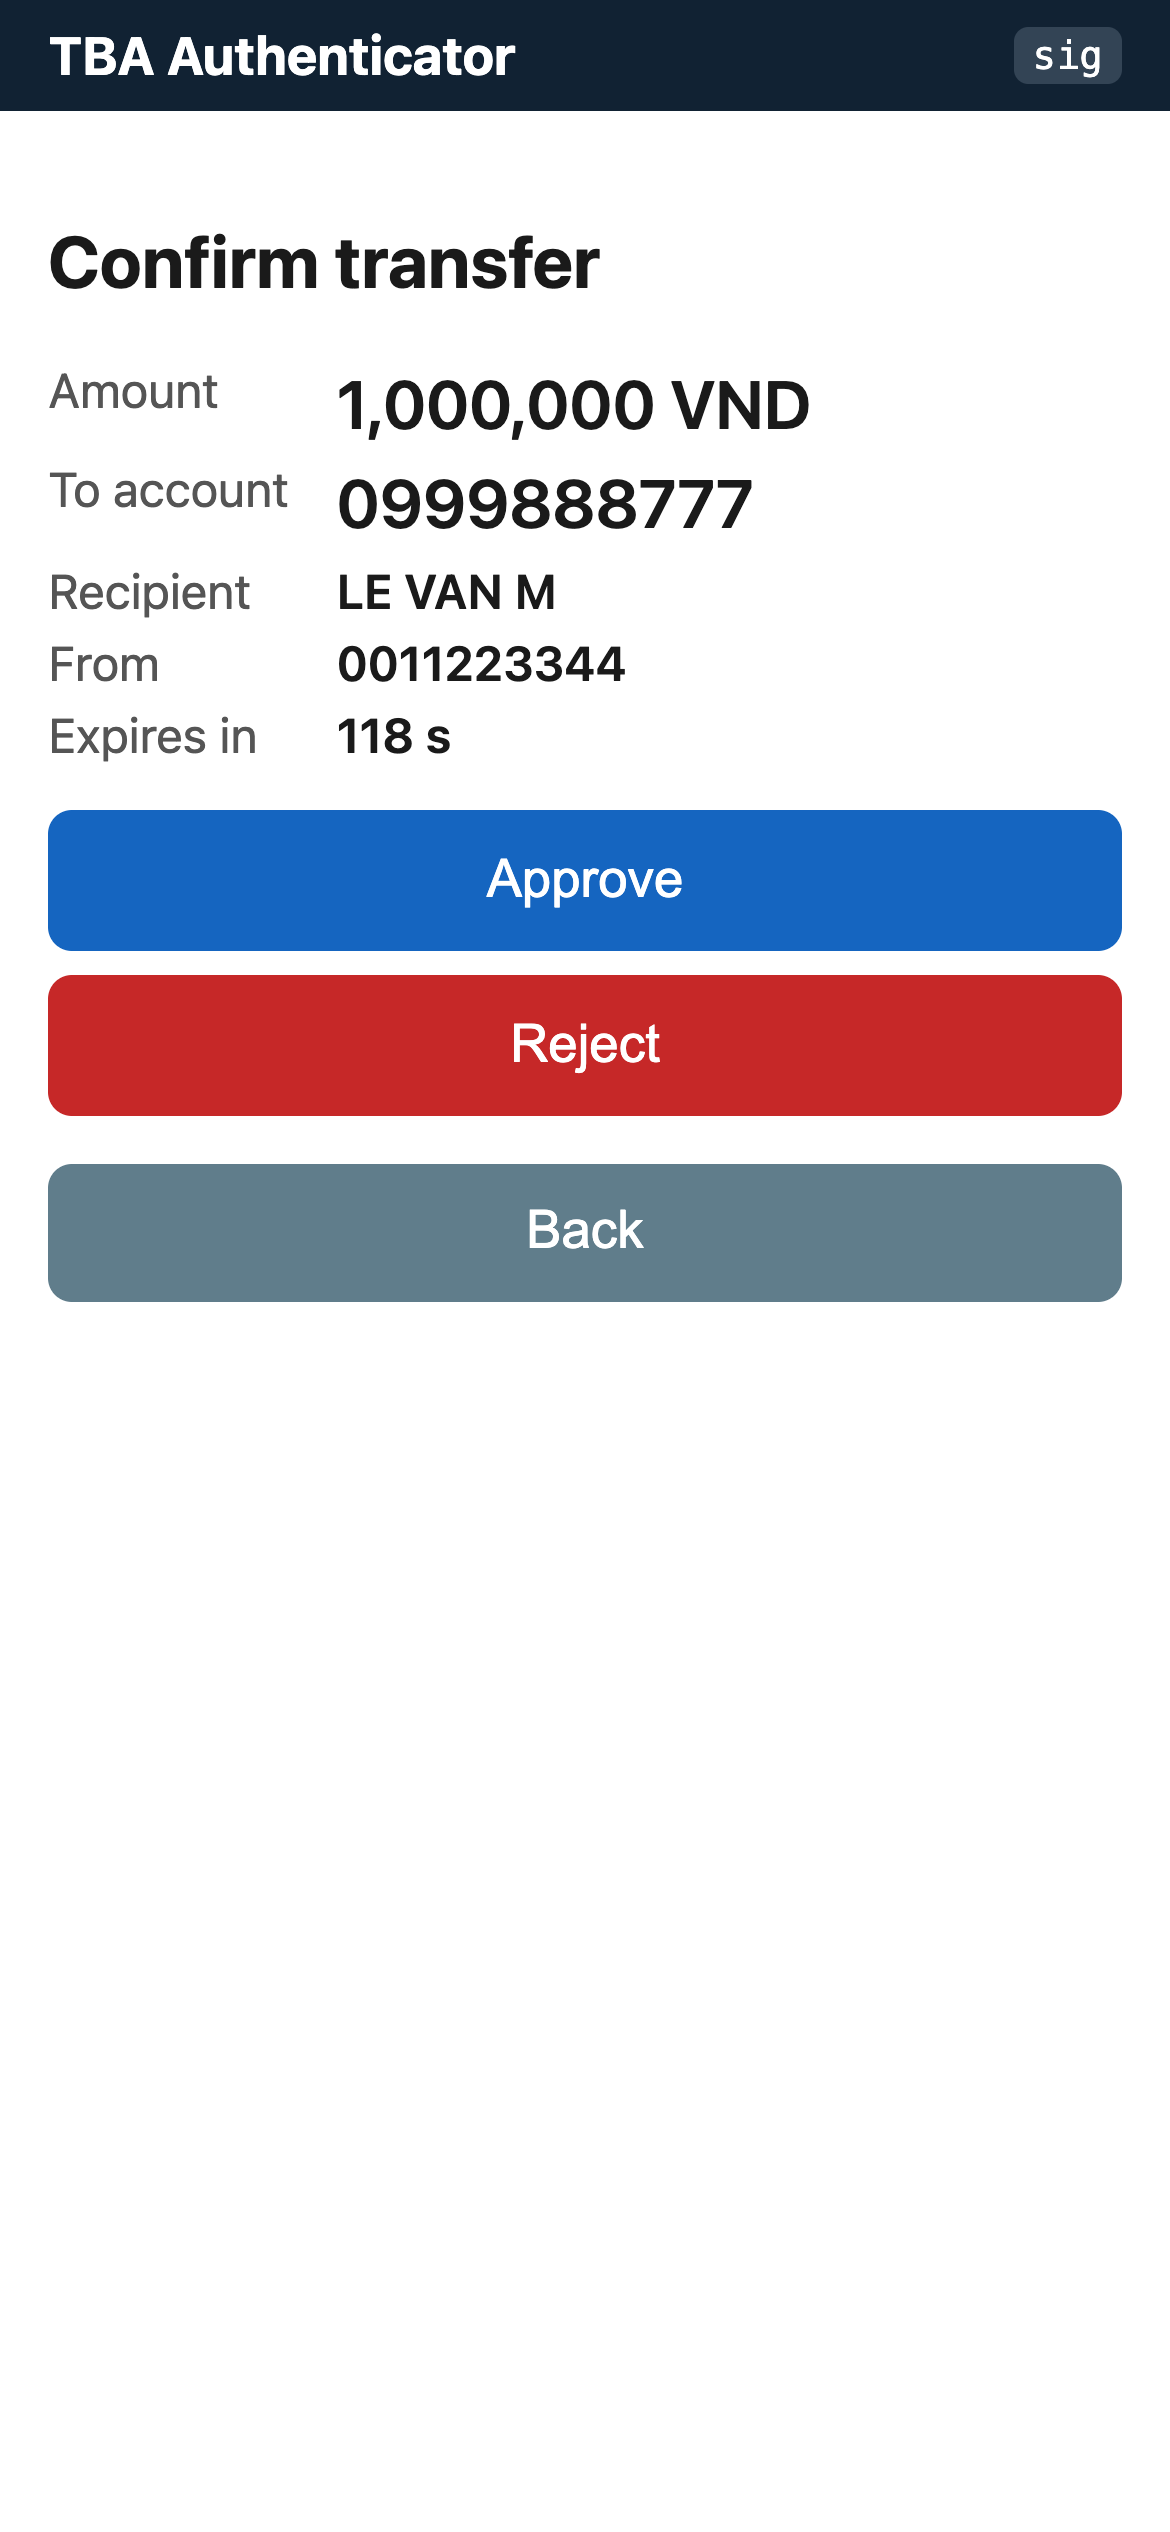
\includegraphics[height=3.4cm]{figures/sig_phone.png}\\ \footnotesize\texttt{sig}
\end{minipage}\hfill
\begin{minipage}{0.3\linewidth}\centering
  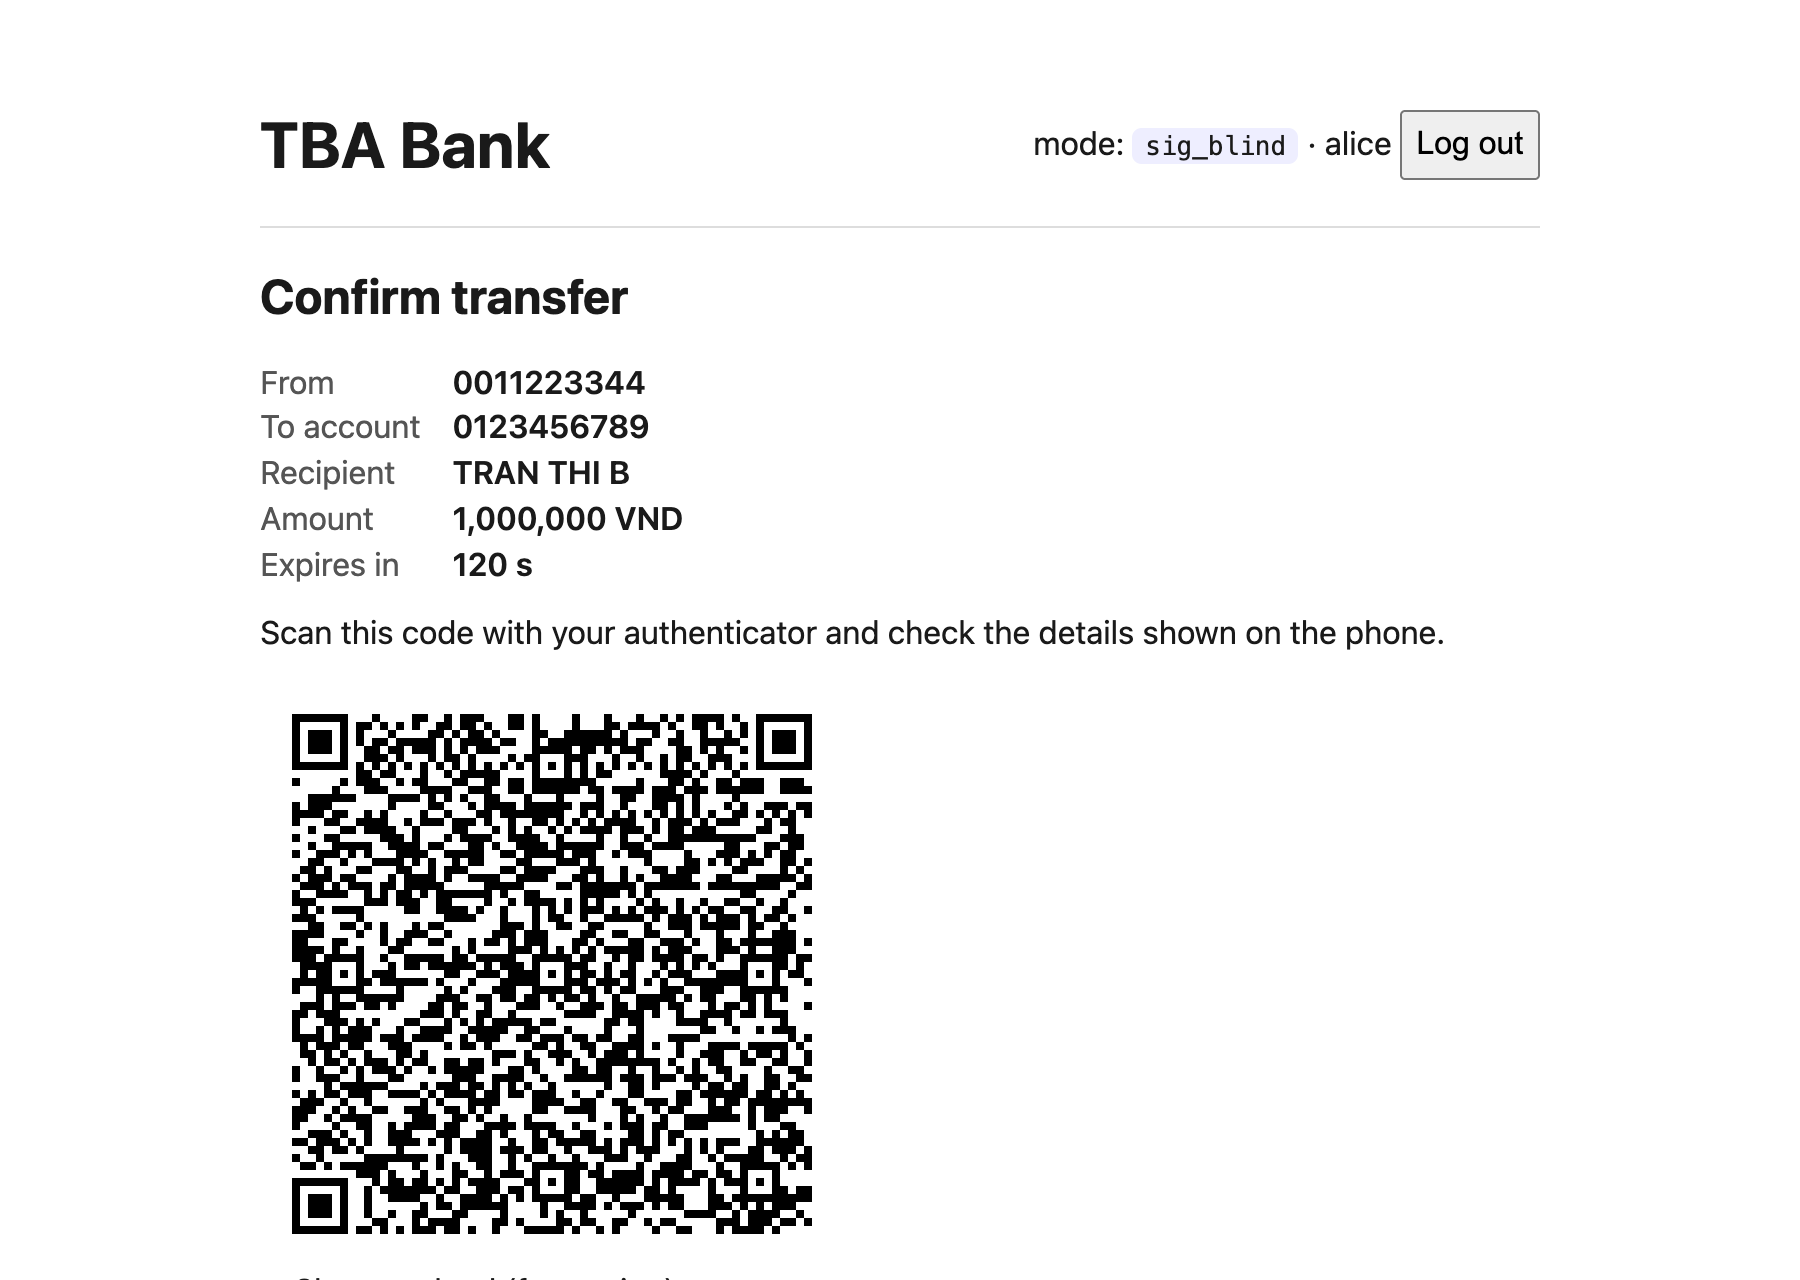
\includegraphics[width=\linewidth]{figures/sig_blind_laptop.png}\\[1mm]
  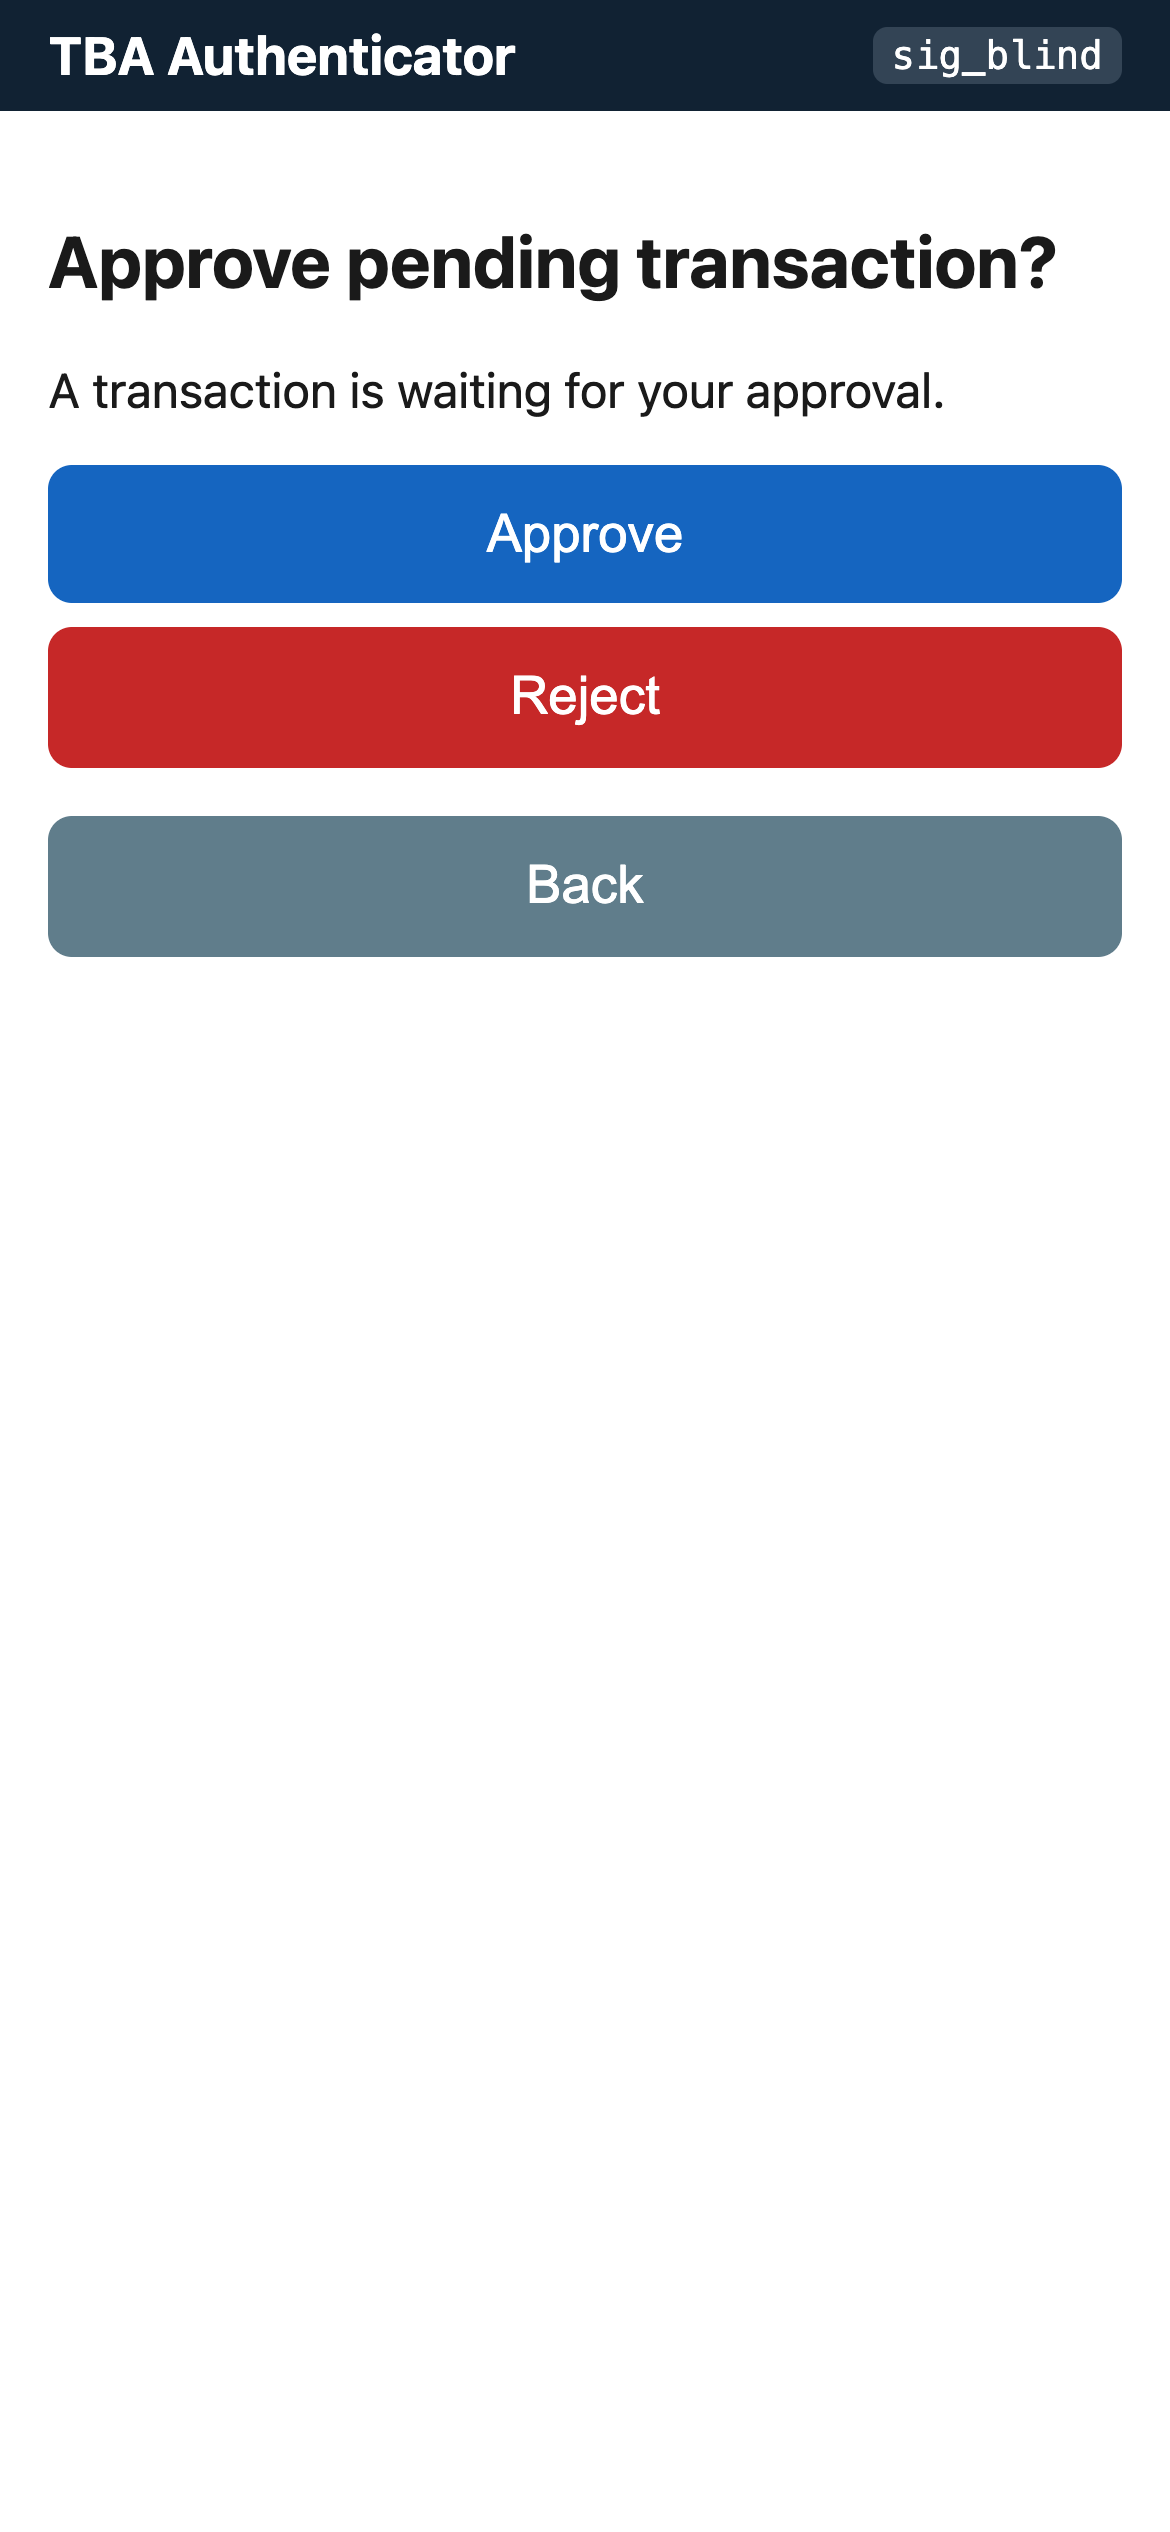
\includegraphics[height=3.4cm]{figures/sig_blind_phone.png}\\ \footnotesize\texttt{sig\_blind}
\end{minipage}
\caption{Live man-in-the-browser. Top row: the laptop confirmation page,
deceived into showing TRAN THI B in every mode. Bottom row: the phone. In
\texttt{hmac}/\texttt{sig} the phone shows the real recipient (0999888777, LE VAN
M); in \texttt{sig\_blind} it shows no details at all.}
\label{fig:mitb}
\end{figure}

\paragraph{RQ2: symmetric versus asymmetric.}
The two differ in S10 and S11, for two distinct reasons. In S10 the leaked
database contains the symmetric keys, so the attacker can compute valid
\texttt{baseline} and \texttt{hmac} codes; it does not contain the ECDSA private
key, so \texttt{sig} survives. In S11 an HMAC code can be checked only by someone
holding the shared key --- which the bank also holds --- whereas a signature can
be verified by anyone with the public key.

\paragraph{RQ3: the display.}
\texttt{sig} and \texttt{sig\_blind} use identical cryptography, yet
\texttt{sig\_blind} fails S2a and S3: with nothing to check, the user approves
the attacker's transaction. S2b is insecure in every mode --- no cryptography
protects a user who approves without looking.

\paragraph{Online guessing.}
Three wrong guesses lock a transaction (S9). A simulation of 100{,}000
transactions matches theory within its 95\% confidence intervals; extrapolated,
the per-transaction success probability is about $9.0\times10^{-6}$ for
\texttt{baseline} (6 digits, three-step window) and $3.0\times10^{-8}$ for
\texttt{hmac} (8 digits). Random forgery of an ECDSA signature is
computationally infeasible.

\section{Discussion and Conclusion}\label{sec:main-conclusion}
\paragraph{Cost.}
The stronger modes are cheap: on the host the median is about $5\,\mu s$ for the
HMAC code and $19\,\mu s$ / $49\,\mu s$ for ECDSA signing / verification, and two
real iPhones sign in $0.29$ and $0.42$~ms on average. The QR payload is 271
characters.

\paragraph{Limitations.}
The \cmark{} cells of S2a, S3 and G7 assume a user who always reads the phone, so
they are an upper bound; we ran no user study. The guessing lockout (G4) is per
transaction only: with no per-user counter, an attacker who knows the password
can spread guesses over $k$ transactions for a chance of about $k\cdot p$
(valid while $k\,p \ll 1$). S11
shows \emph{verifiable evidence}, not non-repudiation, because the bank serves
the authenticator and no independent party attests the public key. The symmetric
keys are stored in plaintext on purpose (an HSM would fix S10 but not S11), and
phone malware (A6) is out of scope.

\paragraph{Conclusion.}
Binding the code to the transaction stops the recipient and amount tampering
that a plain OTP lets through (RQ1). Asymmetric signatures add survival of a
database leak and third-party--verifiable evidence, at under a millisecond per
signature (RQ2). The trusted display is a separate, necessary layer:
\texttt{sig\_blind}, with identical cryptography, fails exactly the attacks an
attentive user would catch (RQ3). No cryptography protects a user who is shown
nothing, or who does not look.
